%%%%%% -*- Coding: utf-8-unix; Mode: latex

%\documentclass[polish]{projectreport}
\documentclass[polish]{projectreport}

\usepackage[utf8]{inputenc}
\usepackage{url}
\usepackage{subfigure}
\usepackage{tabularx}
\usepackage{ragged2e}
\usepackage{booktabs}
\usepackage{multirow}
\usepackage{graphicx}
\usepackage{grffile}

\usepackage[bookmarks=false]{hyperref}
\hypersetup{colorlinks,
  linkcolor=blue,
  citecolor=blue,
  urlcolor=blue}

\usepackage{indentfirst}
\usepackage{caption}
\usepackage{listings}
\usepackage[ruled,linesnumbered,lined]{algorithm2e}
\usepackage[svgnames]{xcolor}
\usepackage{inconsolata}
\usepackage{fancyhdr}

\usepackage{csquotes}
\DeclareQuoteStyle[quotes]{polish}
  {\quotedblbase}
  {\textquotedblright}
  [0.05em]
  {\quotesinglbase}
  {\fixligatures\textquoteright}
\DeclareQuoteAlias[quotes]{polish}{polish}

\usepackage[
style=numeric,
sorting=nyt,
isbn=false,
doi=true,
url=true,
backref=false,
backrefstyle=none,
maxnames=10,
giveninits=true,
abbreviate=true,
defernumbers=false,
backend=biber]{biblatex}
\addbibresource{bibliography.bib}

\lstset{
    %language=Python, %% PHP, C, Java, etc.
    basicstyle=\ttfamily\footnotesize,
    backgroundcolor=\color{gray!5},
    commentstyle=\it\color{Green},
    keywordstyle=\color{Red},
    stringstyle=\color{Blue},
    numberstyle=\tiny\color{Black},    
    % morekeywords={TestKeyword},
    % mathescape=true,
    escapeinside=`',
    frame=single, %shadowbox, 
    tabsize=2,
    rulecolor=\color{black!30},
    title=\lstname,
    breaklines=true,
    breakatwhitespace=true,
    framextopmargin=2pt,
    framexbottommargin=2pt,
    extendedchars=false,
    captionpos=b,
    abovecaptionskip=5pt,
    keepspaces=true,            
    numbers=left,                    
    numbersep=5pt,                  
    showspaces=false,                
    showstringspaces=false,
    showtabs=false,
    tabsize=2
}

\SetAlgorithmName{\LangAlgorithm}{\LangAlgorithmRef}{\LangListOfAlgorithms}

\renewcommand{\lstlistingname}{\LangListing}
\renewcommand\lstlistlistingname{\LangListOfListings}

\newcolumntype{Y}{>{\small\centering\arraybackslash}X}
%\newcolumntype{b}{>{\hsize=1.6\hsize}Y}
%\newcolumntype{m}{>{\hsize=.6\hsize}Y}
%\newcolumntype{s}{>{\hsize=.4\hsize}Y}

\captionsetup[figure]{skip=5pt,position=bottom}
\captionsetup[table]{skip=5pt,position=top}



%%%%%%%%%%%%%%%%%%%%%%%%%%%%%%%%%%%%%%%%%%%%%%%%%%%%%%%%%%%%%%%%%%%%%%%%%%%%%%%
\author{Przemysław Zieliński$^1$  \and Daniel Skowron$^2$ }

\title{Symulacja zachowania tłumu}

\date{
	{\small $^1$Wyższa Szkoła Zarządzania i Bankowości w Krakowie \\ \texttt{przielin@student.wszib.edu.pl}\\[1ex]%
	$^2$Wyższa Szkoła Zarządzania i Bankowości w Krakowie \\ \texttt{daskowra@student.wszib.edu.pl}\\[2ex]%
        \the\year}
      }
      
\pagestyle{fancy}
\fancyhf{}
\fancyhead[LE,RO]{\thepage}

%%%%%%%%%%%%%%%%%%%%%%%%%%%%%%%%%%%%%%%%%%%%%%%%%%%%%%%%%%%%%%%%%%%%%%%%%%%%%%%
\begin{document}

\maketitle

\thispagestyle{empty}

\begin{abstract}
\noindent W pracy przedstawiono zagadnienie symulacji zachowania tłumu oraz zaprojektowano i zaimplementowano mikroskopowy, wieloagentowy model logistyki napływu widzów na stadion. W odróżnieniu od typowych modeli ewakuacyjnych, przedmiotem analizy jest proces \textit{wejścia} kibiców na obiekt, ograniczony przepustowością bramek oraz czasem kontroli biletów. Model zbudowano w języku Python z użyciem frameworka Mesa; ruch agentów wyznaczany jest algorytmem przeszukiwania z heurystyką kosztu uwzględniającą zagęszczenie tłumu. Przeprowadzono cztery serie eksperymentów badających wpływ liczby bramek, ich szerokości, czasu kontroli biletów oraz strategii wyboru bramki na czas zapełnienia trybun i średni czas wejścia. Wyniki pokazują m.in. wyraźny efekt nasycenia --- zwiększanie liczby bramek powyżej progu przestaje skracać czas zapełnienia, gdyż wąskie gardło przenosi się z bramek do korytarzy między rzędami --- oraz nieoczywisty rezultat, w którym kierowanie kibiców do bramki najbliższej ich miejscu wypada gorzej niż wybór bramki najbliższej punktowi wejścia, ze względu na naturalne równoważenie obciążenia bramek w tym drugim przypadku.

\noindent\textbf{Keywords:} symulacja tłumu, modele agentowe (ABM), modelowanie ruchu pieszych, logistyka wejścia na stadion, wąskie gardła, przepustowość, wyznaczanie ścieżki, Mesa, bezpieczeństwo imprez masowych, podejście mikroskopowe.
\end{abstract}

%%%%%%%%%%%%%%%%%%%%%%%%%%%%%%%%%%%%%%%%%%%%%%%%%%%%%%%%%%%%%%%%%%%%%%%%%%%%%%% 
%%%%%%%%%%%%%%%%%%%%%%%%%%%%%%%%%%%%%%%%%%%%%%%%%%%%%%%%%%%%%%%%%%%%%%%%%%%%%%% 
\section{\SectionTitleIntroduction}
\label{sec:introduction}

Symulacja zachowania tłumu to obszar badań, który łączy informatykę z innymi dziedzinami, takimi jak matematyka, fizyka czy socjologia. Współczesne miasta, centra handlowe, stadiony czy stacje metra są miejscami intensywnego przemieszczania się ludzi. W sytuacjach zagrożenia, paniki lub dużego zagęszczenia może dojść do niekontrolowanych zjawisk prowadzących do obrażeń lub ofiar śmiertelnych.

Modelowanie tłumu pozwala analizować bezpieczeństwo ludzi, projektować infrastrukturę oraz planować ewakuację. Zgodnie z \cite{kapalka2011symulacja}, symulacje tłumu znajdują zastosowanie zarówno w analizie sytuacji kryzysowych, jak i w badaniu ruchu pieszych.

W literaturze wyróżnia się dwa główne podejścia do modelowania tłumu: makroskopowe i mikroskopowe. Podejście makroskopowe traktuje tłum jako jednorodny przepływ i opisuje go za pomocą parametrów takich jak gęstość czy średnia prędkość. Podejście mikroskopowe analizuje każdą osobę indywidualnie jako osobny obiekt posiadający własne cele i sposób poruszania się \cite{piwinski2010modelowanie}.

Podejścia mikroskopowe są szczególnie istotne w symulacjach realistycznych, ponieważ pozwalają odwzorować interakcje pomiędzy jednostkami oraz ich reakcje na zmieniające się warunki otoczenia. Jak wskazuje Tąbedzki, modele te uwzględniają m.in. unikanie kolizji, wybór trajektorii ruchu oraz lokalne decyzje podejmowane przez jednostki w czasie rzeczywistym \cite{tabedzki2013mikroskopowe}.

W modelach mikroskopowych często stosuje się systemy agentowe, gdzie każda jednostka jest autonomicznym agentem podejmującym decyzje na podstawie otoczenia. Kapałka proponuje model hybrydowy, łączący reprezentację grafową na poziomie decyzyjnym oraz siatkę komórkową na poziomie ruchu jednostek \cite{kapalka2011symulacja}.

Istotne znaczenie mają także aspekty psychologiczne. Piwiński podkreśla, że człowiek w tłumie zachowuje się inaczej niż indywidualnie --- wzrasta anonimowość, maleje odpowiedzialność, a emocje takie jak strach czy agresja silniej wpływają na decyzje \cite{piwinski2010modelowanie}. Dlatego nowoczesne modele uwzględniają nie tylko fizyczny ruch, ale również relacje społeczne i poziom stresu.

Współczesne badania wykorzystują również Metodę Elementów Dyskretnych (DEM), pozwalającą analizować kolizje, omijanie przeszkód i trajektorie ruchu. Coraz częściej stosuje się także systemy analizy obrazu i monitoring wizyjny do oceny gęstości tłumu oraz wykrywania niebezpiecznych zachowań \cite{piwinski2010modelowanie}.

Obecny kierunek badań zmierza w stronę modeli hybrydowych, łączących podejście fizyczne, psychologiczne i społeczne. Celem niniejszego sprawozdania jest analiza metod symulacji zachowania tłumu oraz przedstawienie modeli wykorzystywanych w badaniu ewakuacji i bezpieczeństwa obiektów użyteczności publicznej.
%%%%%%%%%%%%%%%%%%%%%%%%%%%%%%%%%%%%%%%%%%%%%%%%%%%%%%%%%%%%%%%%%%%%%%%%%%%%%%%



\section{Sformułowanie problemu i proponowane rozwiązanie}
\label{sec:problem_formulation}

\subsection{Opis problemu}
Problem badawczy będący przedmiotem projektu dotyczy modelowania logistyki oraz dynamiki napływu tłumu (inflow) na obiekt masowy, jakim jest stadion. W przeciwieństwie do standardowych modeli ewakuacyjnych, głównym obszarem analizy jest tutaj proces wejścia widzów, poddany rygorom odprawy biletowej oraz przepustowości infrastruktury.

Kluczowym celem jest analiza powstawania tzw. \textit{wąskich gardeł} (bottlenecks) przy wejściach (bramkach) oraz w korytarzach między rzędami siedzeń. Analizie poddane zostaną parametry takie jak czas odprawy biletowej, liczba i szerokość dostępnych bramek wejściowych, a także zachowania samych uczestników (świadomy wybór wejścia dedykowanego w stosunku do poruszania się losowego). Wynikiem symulacji jest optymalizacja zarządzania przepustowością i skrócenie średniego czasu zajmowania miejsc przez przypisanych im kibiców.

\subsection{Model symulacyjny}
Opracowany model funkcjonuje na dyskretnej, dwuwymiarowej siatce (ang. \textit{grid}) o wymiarach 50x50 komórek, korzystając z paradygmatu modelowania wieloagentowego (ABM -- \textit{Agent-Based Modeling}). W przestrzeni modelu współistnieją trzy rodzaje agentów:
\begin{itemize}
    \item \textbf{WallAgent} -- agenci statyczni reprezentujący infrastrukturę fizyczną (ściany, granice trybun), z którymi niemożliwa jest jakakolwiek kolizja czy ich przenikanie przez poruszające się obiekty.
    \item \textbf{SeatAgent} -- statyczni agenci symulujący miejsca dla widzów na trybunach. Przechowują swoje unikalne identyfikatory (rząd i miejsce), stanowiąc punkt docelowy ruchu poszczególnych widzów.
    \item \textbf{FanAgent} -- agenci poruszający się, reprezentujący kibiców. Pojawiają się na obrzeżach symulacji, przechodzą kontrolę przy bramkach, a następnie starają się znaleźć najbardziej optymalną drogę do swojego indywidualnego krzesełka.
\end{itemize}

Standardowo model wymusza obecność maksymalnie jednego agenta na komórce, co sprzyja naturalnemu formowaniu się kolejek. W sytuacjach krytycznych zatorów (tzw. \textit{deadlocków}), algorytm dopuszcza jednak chwilowe zagęszczenie do maksymalnie czterech poruszających się osób na jednym polu, co symuluje zjawisko desperackiego przepuszczania i wymijania się ludzi w skrajnym tłoku. Mechanizm ten jest uruchamiany dopiero po kilku cyklach symulacji (iteracjach), podczas których agent pozostaje zablokowany, co decyzyjnie obrazuje Listing \ref{lst:deadlock}.

\begin{lstlisting}[language=Python, caption={Mechanizm omijania i przeciskania się w przypadku przeciążenia korytarza}, label={lst:deadlock}]
if len(moving_agents) == 0:
    self.model.grid.move_agent(self, next_step)
    self.path.pop(0)
    self.blocked_counter = 0
else:
    self.blocked_counter += 1
    if self.blocked_counter == 3:
        self.path = self.find_path(current_target)
    elif self.blocked_counter > 6:
        if len(moving_agents) < 4:
            self.model.grid.move_agent(self, next_step)
            self.path.pop(0)
            self.blocked_counter = 0
        else:
            self.path = self.find_path(current_target)
            self.blocked_counter = 3
\end{lstlisting}

Podczas symulacji mierzona jest na bieżąco m.in. \textit{Przepustowość} (ilość przepuszczonych kibiców per krok czasowy), \textit{Długość kolejki} oczekującej do skanowania biletów oraz \textit{Średni czas wejścia} informujący po ilu krokach od utworzenia dany kibic zajął swoje miejsce.

\subsection{Algorytmy i biblioteki}

System symulacyjny został zaimplementowany w języku Python przy wykorzystaniu specjalistycznego frameworka \textit{Mesa} przeznaczonego do budowy modeli agentowych\footnote{Pełny kod źródłowy modelu oraz skrypty eksperymentalne dostępne są w repozytorium: \url{https://github.com/daniolsk/symulacja-zachowania-tlumu}}. Do wizualizacji działania tłumu wykorzystano zintegrowany serwer działający na bibliotece \textit{Tornado} (\texttt{mesa\_viz\_tornado}), pozwalający na obserwację ruchu węzłów i rysowanie wykresów analitycznych w czasie rzeczywistym.

Do modelowania przestrzennego nawigowania (ang. \textit{pathfinding}) zastosowano zmodyfikowany algorytm $A^*$ (A-Star) oparty o kolejkę priorytetową (\texttt{heapq}). Trasa każdego kibica wyznaczana jest heurystycznie na podstawie otoczenia Moore'a. Aby zachowanie tłumu było realistyczne, każdy agent weryfikuje gęstość obszaru w zasięgu wzroku przeliczając nową złożoność kroków. 
Funkcja bazowego kosztu wejścia na pole $(x,y)$ obliczana jest zgodnie z poniższym wzorem:

\begin{equation}
    C(x,y) = C_{base} + (N_{crowd} \cdot \beta)
\end{equation}

Gdzie $C$ to całkowity koszt wejścia dla agenta, $C_{base}$ to koszt wejścia uzależniony od infrastruktury ($C_{base} = 1$ dla pustego przejścia oraz $C_{base} = 15$ dla rzędu cudzych krzeseł), a $N_{crowd}$ to liczba innych agentów zidentyfikowana w danej lokalizacji wpływająca na spowolnienie ruchu o wskaźnik $\beta$ (w naszym modelu $\beta = 5$).

W sytuacjach granicznych i przy zablokowaniach (tzw. \textit{deadlockach}), agent porzuca oryginalną ścieżkę szukając obejścia.

%%%%%%%%%%%%%%%%%%%%%%%%%%%%%%%%%%%%%%%%%%%%%%%%%%%%%%%%%%%%%%%%%%%%%%%%%%%%%%%
\section{Wyniki badań eksperymentalnych}
\label{sec:experiments}

\subsection{Metodyka badań}
Eksperymenty przeprowadzono w trybie wsadowym (bez warstwy wizualizacji), uruchamiając model wielokrotnie dla różnych zestawów parametrów. Ze względu na losowość modelu (rozmieszczenie punktów przybycia, przydział miejsc oraz losowa kolejność przeglądania sąsiedztwa w algorytmie ruchu) każdą konfigurację powtarzano niezależnie: trzykrotnie w eksperymentach 2--4 oraz ośmiokrotnie w eksperymencie dotyczącym liczby bramek (z uwagi na większą zmienność wyników). Prezentowane wartości stanowią uśrednienie po replikacjach, a w eksperymencie z liczbą bramek --- medianę.

Jako główne miary efektywności przyjęto czas zapełnienia oraz średni czas wejścia:
\begin{itemize}
    \item \textbf{Czas zapełnienia} --- liczbę kroków symulacji potrzebną do zajęcia miejsc przez \emph{wszystkich} kibiców (miara przepustowości całego procesu);
    \item \textbf{Średni czas wejścia} --- średnią liczbę kroków, po której pojedynczy kibic zajmuje swoje miejsce (miara sprawności procesu z perspektywy pojedynczego widza).
\end{itemize}
Pomocniczo rejestrowano również \textbf{długość kolejki} (liczbę kibiców oczekujących na odprawę), której przebieg w czasie prezentuje panel metryk warstwy wizualizacyjnej (Rysunek~\ref{fig:live_charts}).

We wszystkich eksperymentach zmieniano tylko jeden badany parametr, pozostałe utrzymując na wartościach bazowych: 200 kibiców, 4 bramki, szerokość bramki 2 komórki, czas kontroli biletu 5 kroków oraz świadomy wybór bramki. Odstępstwa od tej konfiguracji (np. zmniejszone obciążenie w eksperymencie 2. czy zmienną liczbę kibiców w eksperymencie 4.) zaznaczono w opisie poszczególnych badań.

Poglądowy przebieg symulacji przedstawia Rysunek~\ref{fig:sim_overview}: widoczni są kibice oczekujący w kolejce (kolor czerwony), przechodzący kontrolę biletową przy bramce (kolor żółty) oraz zajmujący już swoje miejsca (kolor zielony). Rysunek~\ref{fig:bottleneck} ilustruje natomiast zjawisko wąskiego gardła powstające przy ograniczeniu liczby bramek do jednej.

\begin{figure}[htbp]
    \centering
    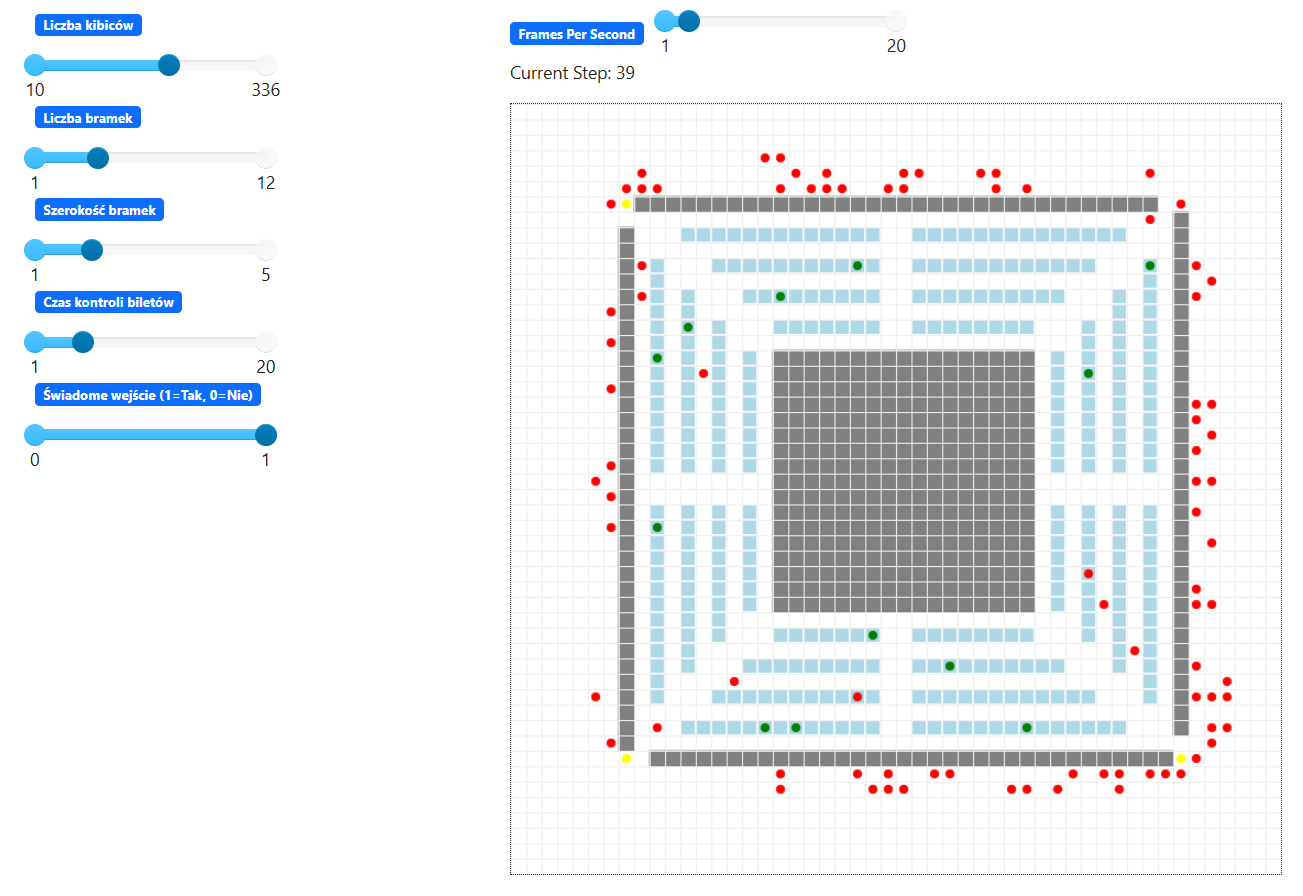
\includegraphics[width=0.7\textwidth]{experiments/plots/rys_symulacja_ogolna.png}
    \caption{Ogólny widok symulacji w trakcie napływu widzów. Czerwone znaczniki --- kibice w kolejce, żółte --- w trakcie kontroli biletów, zielone --- zajmujące miejsca.}
    \label{fig:sim_overview}
\end{figure}

\begin{figure}[htbp]
    \centering
    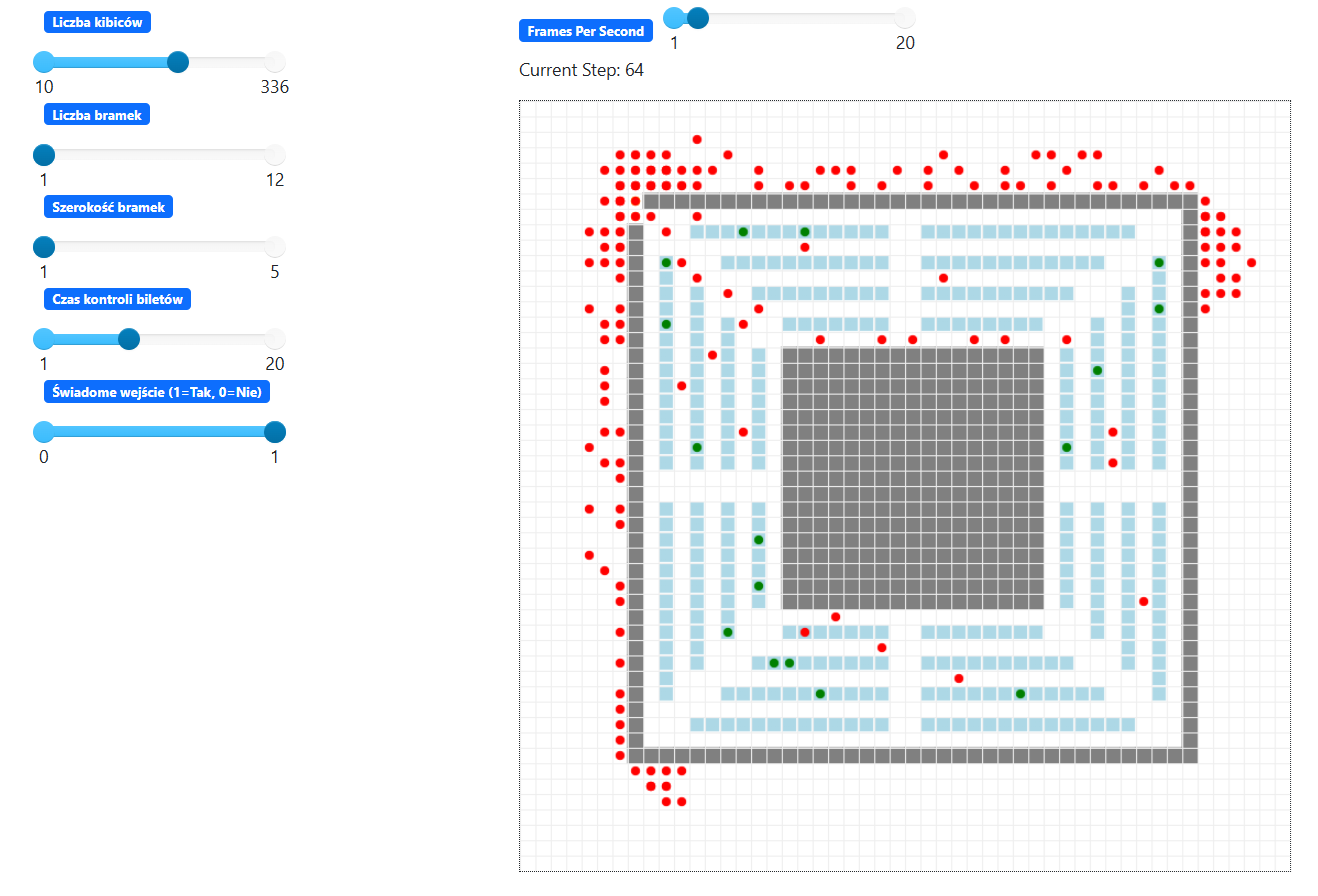
\includegraphics[width=0.7\textwidth]{experiments/plots/rys_waskie_gardlo.png}
    \caption{Zjawisko wąskiego gardła (\textit{bottleneck}) --- pojedyncza bramka powoduje formowanie się długiej kolejki i znaczne wydłużenie czasu wejścia.}
    \label{fig:bottleneck}
\end{figure}

Warstwa wizualizacji na bieżąco prezentuje również wykresy trzech mierzonych metryk (Rysunek~\ref{fig:live_charts}), co pozwala śledzić dynamikę procesu napływu w czasie rzeczywistym.

\begin{figure}[htbp]
    \centering
    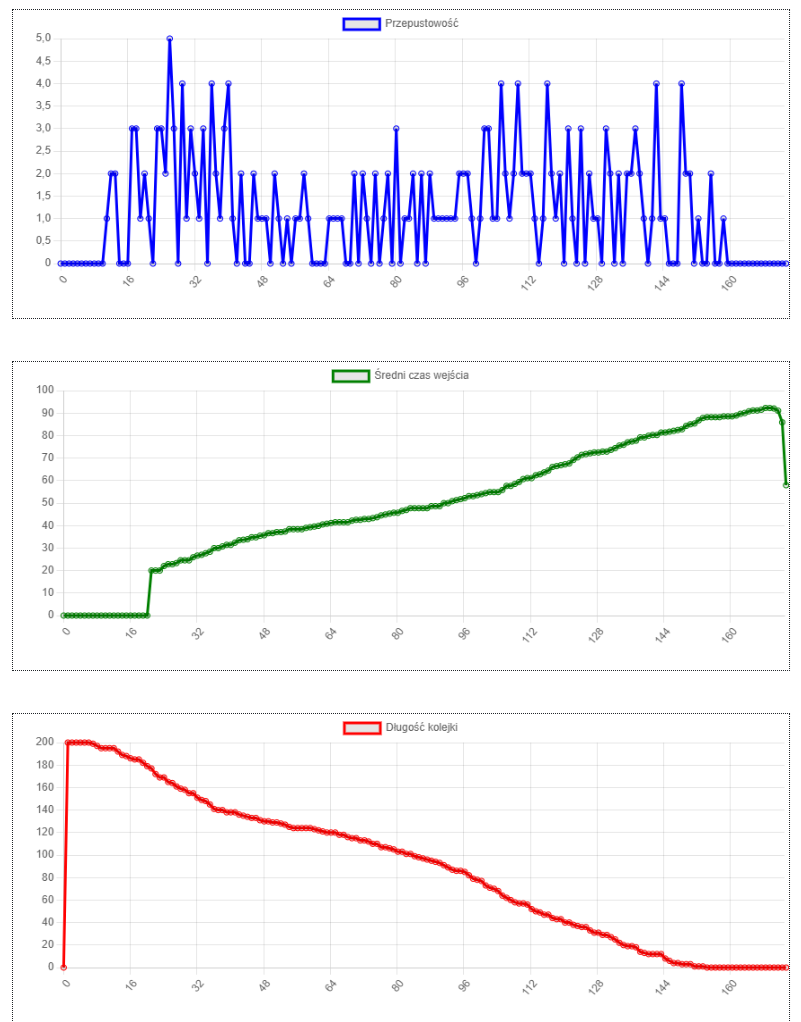
\includegraphics[width=0.7\textwidth]{experiments/plots/rys_wykresy_live.png}
    \caption{Panel metryk w czasie rzeczywistym: przepustowość, średni czas wejścia oraz długość kolejki w kolejnych krokach symulacji.}
    \label{fig:live_charts}
\end{figure}

\subsection{Eksperyment 1: wpływ liczby bramek}
W pierwszym eksperymencie badano wpływ liczby bramek wejściowych na przepustowość obiektu przy stałym obciążeniu 200 kibiców. Ze względu na to, że przy małej liczbie bramek pojawiały się sporadyczne, długotrwałe zatory, każdą konfigurację powtórzono 8~razy, a jako główną miarę przyjęto \emph{medianę} czasu zapełnienia (odporną na pojedyncze biegi niezakończone w limicie kroków). Wyniki zestawiono w Tabeli~\ref{tab:gates} oraz na Rysunku~\ref{fig:exp1}.

\begin{table}[htbp]
    \centering
    \caption{Wpływ liczby bramek (200 kibiców). Kolumna „Ukończone'' podaje, w ilu z~8 biegów wszyscy kibice zajęli miejsca przed osiągnięciem limitu kroków.}
    \label{tab:gates}
    \begin{tabular}{@{}rrrr@{}}
        \toprule
        Liczba bramek & Mediana czasu zapełnienia [kroki] & Średni czas wejścia [kroki] & Ukończone \\
        \midrule
        1 & 292 & 156 & 8/8 \\
        2 & 192 & 104 & 7/8 \\
        3 & 183 & 99  & 7/8 \\
        4 & 176 & 94  & 8/8 \\
        6 & 172 & 93  & 8/8 \\
        8 & 169 & 92  & 8/8 \\
        \bottomrule
    \end{tabular}
\end{table}

\begin{figure}[htbp]
    \centering
    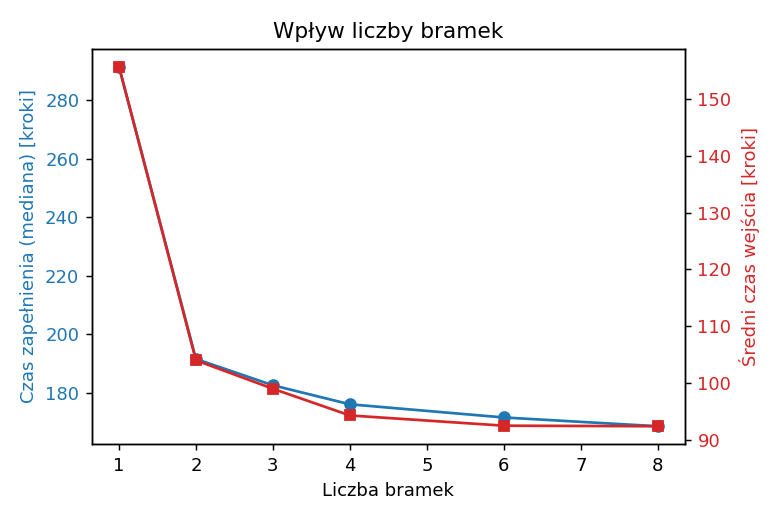
\includegraphics[width=0.65\textwidth]{experiments/plots/exp1_gates.png}
    \caption{Zależność mediany czasu zapełnienia oraz średniego czasu wejścia od liczby bramek.}
    \label{fig:exp1}
\end{figure}

Zaobserwowano wyraźny \emph{efekt nasycenia}. Przejście z jednej do dwóch bramek skraca medianę czasu zapełnienia o ok. 34\% (z 292 do 192 kroków), a średni czas wejścia o ok. jedną trzecią (ze 156 do 104 kroków). Dalsze zwiększanie liczby bramek przynosi już tylko marginalne korzyści --- powyżej 4 bramek krzywa spłaszcza się na poziomie ok. 170 kroków. Oznacza to, że po odblokowaniu wejść czynnikiem ograniczającym przestają być same bramki, a staje się nim wewnętrzna infrastruktura (korytarze i dojścia do rzędów siedzeń). Dodatkowo, przy 2--3 bramkach jeden na osiem biegów nie rozładował się w pełni w zadanym limicie kroków --- świadczy to o tym, że przy umiarkowanej liczbie wejść model bywa podatny na przejściowe zakleszczenia w wąskich korytarzach (por. ograniczenia modelu w Rozdziale~\ref{sec:conclusions}).

\subsection{Eksperyment 2: wpływ czasu kontroli biletów}
W eksperymencie badano wpływ czasu odprawy biletowej (liczby kroków potrzebnych na przeskanowanie jednego biletu) na przepustowość procesu. Ze względu na to, że długi czas kontroli drastycznie wydłuża biegi symulacji, obciążenie ustalono na poziomie 120 kibiców. Wyniki zebrano w Tabeli~\ref{tab:service} oraz na Rysunku~\ref{fig:exp2}.

\begin{table}[htbp]
    \centering
    \caption{Wpływ czasu kontroli biletów (120 kibiców, 4 bramki).}
    \label{tab:service}
    \begin{tabular}{@{}rrr@{}}
        \toprule
        Czas kontroli [kroki] & Czas zapełnienia [kroki] & Średni czas wejścia [kroki] \\
        \midrule
        1  & 136 & 77 \\
        3  & 144 & 74 \\
        5  & 150 & 80 \\
        8  & 154 & 86 \\
        12 & 164 & 93 \\
        \bottomrule
    \end{tabular}
\end{table}

\begin{figure}[htbp]
    \centering
    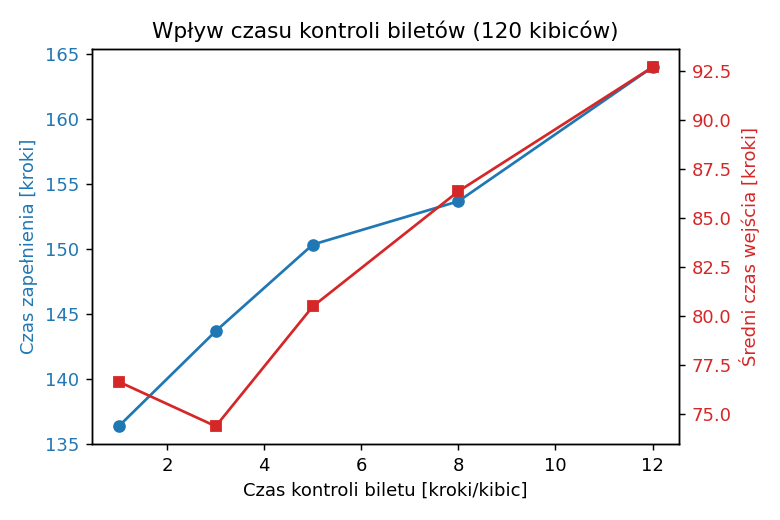
\includegraphics[width=0.65\textwidth]{experiments/plots/exp2_service.png}
    \caption{Zależność czasu zapełnienia i średniego czasu wejścia od czasu kontroli biletu.}
    \label{fig:exp2}
\end{figure}

Zaobserwowano niemal liniowy wzrost zarówno czasu zapełnienia trybun (ze 136 do 164 kroków, tj. o ok. 21\%), jak i średniego czasu wejścia pojedynczego kibica (z ok. 77 do 93 kroków) wraz z wydłużaniem procedury kontroli. Wynik ten potwierdza intuicję, że odprawa biletowa jest jednym z kluczowych, sterowalnych elementów wąskiego gardła --- każde skrócenie czasu obsługi (np. przez automatyzację skanowania) bezpośrednio przekłada się na szybszy i płynniejszy napływ widzów.

\subsection{Eksperyment 3: wpływ szerokości bramek}
Kolejny eksperyment dotyczył szerokości bramek, tj. liczby komórek, przez które równolegle może odbywać się odprawa w obrębie jednej bramki. Wyniki przedstawia Tabela~\ref{tab:width} oraz Rysunek~\ref{fig:exp3}.

\begin{table}[htbp]
    \centering
    \caption{Wpływ szerokości bramek (200 kibiców, 4 bramki).}
    \label{tab:width}
    \begin{tabular}{@{}rrr@{}}
        \toprule
        Szerokość bramki & Czas zapełnienia [kroki] & Średni czas wejścia [kroki] \\
        \midrule
        1 & 182 & 102 \\
        2 & 175 & 99 \\
        3 & 167 & 92 \\
        4 & 167 & 91 \\
        5 & 172 & 91 \\
        \bottomrule
    \end{tabular}
\end{table}

\begin{figure}[htbp]
    \centering
    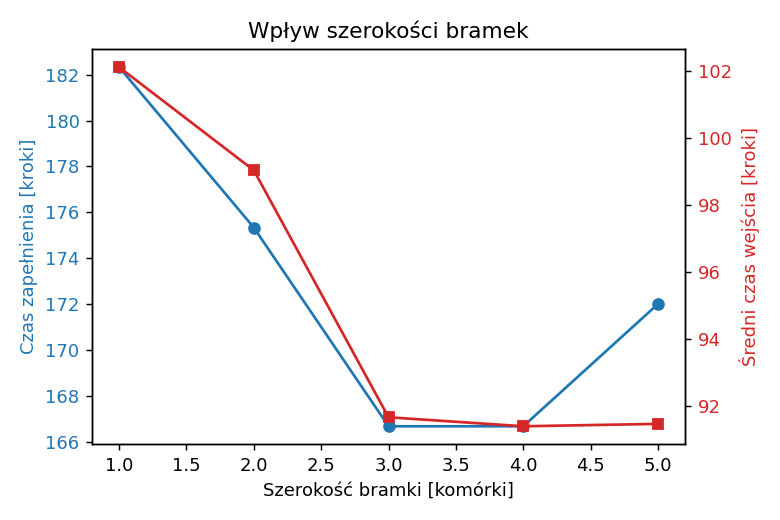
\includegraphics[width=0.65\textwidth]{experiments/plots/exp3_width.png}
    \caption{Zależność czasu zapełnienia i średniego czasu wejścia od szerokości bramek.}
    \label{fig:exp3}
\end{figure}

Poszerzanie bramek przynosi umiarkowaną poprawę: przejście od szerokości 1 do 3 komórek skraca czas zapełnienia o ok. 8\% (ze 182 do 167 kroków) i średni czas wejścia o ok. 10\%. Powyżej szerokości 3 komórek efekt się nasyca, a dla szerokości 5 obserwujemy nawet nieznaczne pogorszenie. Wskazuje to, że sama zdolność przepustowa bramek przestaje być czynnikiem ograniczającym --- po jej odblokowaniu przepustowość całości limitowana jest już przez korytarze i dojścia do rzędów siedzeń.

\subsection{Eksperyment 4: świadomy vs losowy wybór bramki}
Ostatni eksperyment porównywał dwie strategie wyboru bramki przez kibica w funkcji obciążenia obiektu (od 100 do 300 osób):
\begin{itemize}
    \item \textbf{Świadome wejście} --- kibic kieruje się do bramki położonej najbliżej swojego \emph{miejsca} na trybunie;
    \item \textbf{Losowe (naturalne) wejście} --- kibic kieruje się do bramki położonej najbliżej swojego \emph{punktu przybycia}.
\end{itemize}

\begin{table}[htbp]
    \centering
    \caption{Porównanie strategii wyboru bramki. Wartości: średni czas wejścia / czas zapełnienia [kroki].}
    \label{tab:smart}
    \begin{tabular}{@{}rcc@{}}
        \toprule
        Liczba kibiców & Świadome wejście & Losowe wejście \\
        \midrule
        100 & 81 / 139 & 66 / 113 \\
        150 & 88 / 160 & 79 / 139 \\
        200 & 94 / 174 & 86 / 153 \\
        250 & 102 / 192 & 97 / 176 \\
        300 & 113 / 199 & 103 / 190 \\
        \bottomrule
    \end{tabular}
\end{table}

\begin{figure}[htbp]
    \centering
    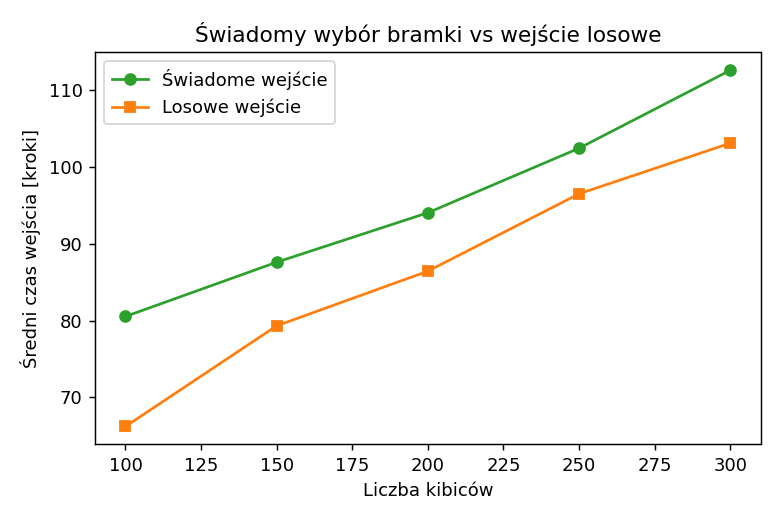
\includegraphics[width=0.65\textwidth]{experiments/plots/exp4_smart.png}
    \caption{Średni czas wejścia dla strategii świadomego oraz losowego wyboru bramki w funkcji liczby kibiców.}
    \label{fig:exp4}
\end{figure}

Wyniki (Tabela~\ref{tab:smart}, Rysunek~\ref{fig:exp4}) okazały się nieoczywiste: strategia \emph{losowa} okazała się konsekwentnie szybsza od strategii \emph{świadomej} --- średni czas wejścia był krótszy o ok. 8--18\% w całym zakresie obciążenia. Wyjaśnienie tego zjawiska jest emergentną własnością modelu. Kierowanie się do bramki najbliższej punktowi przybycia w naturalny sposób \emph{równoważy obciążenie} wszystkich bramek (kibice przybywający z różnych stron rozkładają się równomiernie) oraz minimalizuje drogę pokonywaną wzdłuż zewnętrznego obwodu obiektu. Z kolei kierowanie się do bramki najbliższej miejscu na trybunie prowadzi do lokalnych spiętrzeń --- kibice o miejscach skupionych w jednym sektorze tłoczą się przy tej samej bramce --- oraz wymusza dłuższe przemieszczanie się na zewnątrz stadionu. Wniosek praktyczny: przy projektowaniu organizacji wejść korzystniejsze bywa rozproszenie strumienia widzów na najbliższe dostępne wejścia niż sztywne przypisanie sektorów do bramek.

%%%%%%%%%%%%%%%%%%%%%%%%%%%%%%%%%%%%%%%%%%%%%%%%%%%%%%%%%%%%%%%%%%%%%%%%%%%%%%%
\section{Podsumowanie i wnioski}
\label{sec:conclusions}

W ramach projektu zaprojektowano i zaimplementowano mikroskopowy, wieloagentowy model symulacyjny logistyki napływu widzów na stadion. Model, zbudowany w języku Python z wykorzystaniem frameworka Mesa, odwzorowuje kluczowe elementy procesu wejścia: przybycie kibiców, kontrolę biletową przy bramkach o zadanej liczbie i szerokości, nawigację do przypisanego miejsca z omijaniem przeszkód i tłoku, a także naturalne formowanie się kolejek i chwilowych zatorów.

Przeprowadzone eksperymenty pozwoliły sformułować następujące wnioski:
\begin{itemize}
    \item \textbf{Liczba bramek} jest najsilniejszym czynnikiem wpływającym na przepustowość przy małych wartościach, jednak jej zwiększanie wykazuje wyraźny \emph{efekt nasycenia}. Powyżej progu kilku bramek wąskie gardło przenosi się z wejść do wewnętrznej infrastruktury (korytarzy i dojść do rzędów), a dalsza rozbudowa liczby bramek przestaje skracać czas zapełnienia.
    \item \textbf{Czas kontroli biletów} wpływa na czas zapełnienia i średni czas wejścia w sposób niemal liniowy. Jest to najłatwiej sterowalny parametr organizacyjny --- inwestycja w szybszą odprawę (np. bramki automatyczne) daje bezpośredni zysk czasowy.
    \item \textbf{Szerokość bramek} poprawia przepustowość jedynie do pewnego progu, po którym czynnikiem ograniczającym stają się elementy wewnętrzne obiektu.
    \item \textbf{Strategia wyboru bramki} ma istotne znaczenie, przy czym --- wbrew intuicji --- rozproszenie widzów na wejścia najbliższe punktowi przybycia (równoważące obciążenie) przewyższa sztywne kierowanie ich do bramki przy własnym sektorze.
\end{itemize}

Nadrzędnym wnioskiem płynącym z badań jest obserwacja, że przepustowość obiektu masowego jest wypadkową \emph{całego łańcucha} elementów, a optymalizacja pojedynczego z nich (np. dodawanie bramek) napotyka na barierę wynikającą z przeniesienia się wąskiego gardła w inne miejsce. Efektywne zarządzanie napływem wymaga zatem równoległego uwzględnienia przepustowości bramek, czasu odprawy, geometrii korytarzy oraz sposobu rozkładania strumienia ludzi.

Model posiada naturalne ograniczenia: jest dyskretny (siatka), abstrahuje od indywidualnych prędkości i czynników psychologicznych (panika, zachowania stadne), a mechanizm rozwiązywania zatorów w rzadkich przypadkach nie doprowadza do pełnego rozładowania ruchu przy niewielkiej liczbie bramek. Kierunkami dalszego rozwoju są: wprowadzenie zróżnicowanych profili zachowań agentów, uwzględnienie modelu sił społecznych, buforowanie wyznaczonych ścieżek w celu przyspieszenia symulacji większych tłumów oraz rozszerzenie analizy o scenariusze ewakuacji (odwrócenie kierunku przepływu).

%%%%%%%%%%%%%%%%%%%%%%%%%%%%%%%%%%%%%%%%%%%%%%%%%%%%%%%%%%%%%%%%%%%%%%%%%%%%%%%


\printbibliography
%%%%%%%%%%%%%%%%%%%%%%%%%%%%%%%%%%%%%%%%%%%%%%%%%%%%%%%%%%%%%%%%%%%%%%%%%%%%%%%
\end{document}
